\section{Background}
\label{sec:background}

%Component-based engineering, UML state machine, round-trip engineering

This section reminds the background definitions of UML State Machine (see \ref{subsec:usmbackground}) and Model-Driven Round-Trip Engineering (see \ref{subsec:mdrtebackground}) in a formal way.


\subsection{UML State Machine}
\label{subsec:usmbackground}
%\begin{definition}A directed graph $G = \{V, Ed\}$ consists of a finite set $V$ of vertexes, and a set $Ed$ of edges. An edge connects a source vertex to a target vertex. The source and target vertexes of an edge ed are obtained by $src(ed)$ and $tgt(ed)$.
%\end{definition}

%This section presents the background of UML State Machine whose meta-model is shown in
 Fig. \ref{fig:smmetamodel} shows the meta-model of UML State Machine whose detailed semantics is clearly defined in the Precise Semantics for UML State Machine specification \cite{OMG2015} and beyond the scope of this paper.
%Fig. \ref{fig:smmetamodel} shows the state machine meta-model used in this paper.
This meta-model covers all concepts defined by UML State Machine.
The behavior of an \ttt{ActiveClass} is described by a state machine\footnote{%It is possible to have multiple state machines in the same active class. However, 
	For simplification, this paper assumes that an active class only holds a USM although it can have more}.
%Furthermore, instead of using the \ttt{Behavior} UML meta-element, we introduce \ttt{Action} to define actions of state and transition, which actually are user-code.
%\ttt{Action} is convenient in many modeling tools such as IBM Rhapsody and Enterprise Architect to allow the developers to write the low level code (user-code) directly at the model level.
%The user-code is then printed in the generated code.
%\begin{definition}A UML vertex $v \in V$ has a kind $v.kind \in$  \ti{\{initial, final, state, comp, conc, join, fork, choice, junction, enpoint, expoint, history\}}. 
%\end{definition} 
%\begin{definition} 
A transition connects two vertexes. %, \ttt{source} and \ttt{target}. 
%The source and target vertexes of an edge ed are obtained by $src(t)$ and $tgt(t)$. 
It can have a $guard$, an $effect$, and is triggered by a set of events. 
%We write $events(t)$ as the associated set of events. 
A transition 
%has a type $t.type$ $\in \{trig, tless, gdless, triggdless\}$ and a 
is either \ttt{external}, \ttt{local}, or \ttt{internal}. %whose semantics is defined by the specification.
%\end{definition}
UML defines five event types. 
%Fig. \ref{fig:eventmetamodel} shows the meta-model of the event types.
The description of the events is briefly stated as the following.


%\begin{definition}A region $r \in \mathcal{R}$ is composed of one or several vertexes, and contained by a state $s$. We write $owner(r) = s$ and $vertices(r)$ is its sub-vertices set. 
%\end{definition}	
\begin{comment} 
	A vertex is either a UML state or a pseudo-state. 
	A state can be either \ttt{simple}, \ttt{composite}, or \ttt{orthogonal/concurrent}. 
	%if it contains at least one region; \ttt{orthogonal/concurrent} if contains more than one region; otherwise \ttt{simple}. 
	A state can have an $entry$, an $exit$ and a $doActivity$ action. 
	%A composite state $cs$ contains one or more vertexes. 
	%We write $vertices(cs)$ is a set of vertexes contained by $cs$ and, inversely, $owner(v)$ refers to the containing state of the vertex $v$. 
	%A vertex is a pseudo state if it is not a state.
	A connection point is a vertex, whose kind $\in \{enpoint, expoint\}$, and contained by a composite/concurrent state.%A concurrent state contains more than one region.
\end{comment}		
%A vertex \ttt{v} is either contained by a region, which is in turn contained by a state or a state machine, or a state if it is a \ttt{connection point}, \ttt{v} is called a sub-vertex of the state or state machine.




%\begin{definition} An action $act$ $\in$ $ActLang$ is a set of statements written in an object-oriented programming language $ActLang$. A guard is a boolean expression written in $ActLang$.
%\end{definition}


\begin{figure}
	\centering
	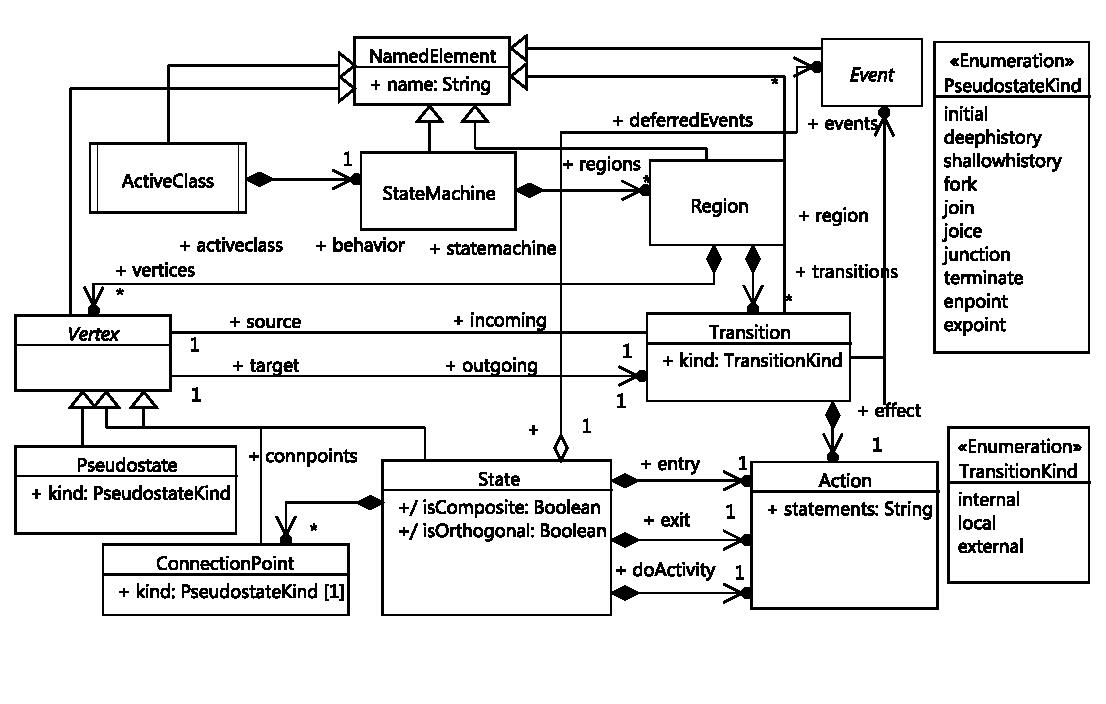
\includegraphics[clip, trim=0.2cm 1.5cm 0.2cm 0.5cm, width=1.0\columnwidth]{figures/smmetamodel.pdf}
	\caption{State machine meta-model} 
	\label{fig:smmetamodel}
\end{figure}



%\begin{definition} An event is one of the followings:
	\begin{itemize}[\footnotesize]
		\item A \ttt{TimeEvent} specifies the time of occurrence \ttt{dur} relative to a starting time. 
		The latter is specified as the time when a state, which accepts the time event, is entered.
		
		\item A \ttt{SignalEvent} is associated with a signal \ttt{sig}, whose data are described by its attributes, and occurs if \ttt{sig} is received by a component, which is an active UML class.
		
		\item A \ttt{ChangeEvent} is associated with a boolean expression \ttt{expr}. \ttt{ChangeEvent} is emitted if the value of \ttt{expr} changes from false to true.
		
		\item A \ttt{CallEvent} is associated with an operation \ttt{op}. 
		\ttt{CallEvent} is emitted if there is an invocation to \ttt{op}.
		
		\item An \ttt{Any} event is any of the above events.
	\end{itemize}
%\end{definition}

\begin{comment}
\begin{figure}
	\centering
	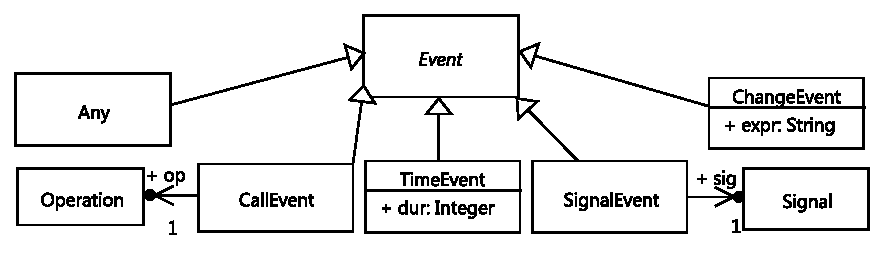
\includegraphics[clip, trim=0.2cm 0.2cm 0.2cm 0.2cm, width=1.0\columnwidth]{figures/eventmetamodel.pdf}
	\caption{State machine event meta-model} 
	\label{fig:eventmetamodel}
\end{figure}
\end{comment}

\begin{comment}
\begin{definition} A \ti{TimeEvent} $te$ an internal event and specifies the time of occurrence $d$ relative to a starting time. The latter is specified when a state, which accepts the time event, is entered. 
\end{definition}

\begin{definition} A \ti{Signal} $sig$ is data described by its attributes. 
\end{definition}

\begin{definition} A \ti{SignalEvent} $se$ is associated with a signal $sig$ and is occurred if $sig$ is received by a component, which is an active UML class. 
\end{definition}	

\begin{definition}
	A \ti{ChangeEvent} $che$ is associated with a boolean expression $ex(che)$ written in $ActLang$. $che$ is emitted if $ex(che)$ changes from true (false) to false (true).
\end{definition}

\begin{definition}
	A \ti{CallEvent} $ce$ is associated with an operation $op(ce)$. $ce$ is emitted if there is a call to $op(ce)$.
\end{definition}
\end{comment}

%Suppose that for each vertex \ti{v} $\in$ $V$, its incoming and outgoing transition lists are extracted by $T_{ins}(v)$ and $T_{outs}(v)$, respectively. %For a list $l$, the function $head$ is used to get the first element of the list. 
%If $v.kind = conc$, suppose $regions(v)$ is the region set contained by $v$. %Given a transition t:
%\begin{itemize}
%	\item $t.type = trig$ if $\#events(t) > 0$.
%	\item $t.type = tless$ if $\#events(t) = 0$.
%	\item $t.type = gdless$ if $(guard(t) = true \vee \nexists guard(t)$.
%	\item $t.type = triggdless$ if $\#events(t) = 0 \wedge (guard(t) = true \vee \nexists guard(t))$.
%\end{itemize}

%The behavior of an active class $C$ is described by using a state machine whose definition is as following:	

%\begin{definition} A state machine sm is a graph specified by $\{V, T, E\}$ with $E$ as a set of events. 
%	A state machine is a special composite state which has no incoming and no outgoing transitions. 
%	A root vertex $v$ is a direct sub-vertex of the state machine, $owner(v) = sm$. The set of regions contained by $sm$ is written $\mathcal{R}$.
%\end{definition}	

%For each vertex $v$ $\in$ $V$, we write the following sets $T_{ins} (v) = incomings(v), T_{outs}(v) = outgoings(v)$, $t_{first} = head(t_{outs})$; transitive transition sets $T_{ins}^{+}(v)$ and $T_{outs}^{+}(v)$ are sets of transitions incoming to and outgoing from, respectively, $v$ or direct or indirect sub-vertexes of $v$.

\begin{comment}
\begin{strip}
	\begin{equation}
	T_{ins}^{+} (v) =    \left\{
	\begin{array}{ll}
	T_{ins}(v) & v.kind \notin \{comp, conc\}  \\
	T_{ins}(v) \cup \bigcup\limits_{sub \in subvertexes(v)} T_{ins}^{+} (sub) & v.kind \in \{comp, conc\} \\
	\end{array} 
	\right.
	\end{equation}
	
	\begin{equation}
	T_{outs}^{+} (v) =    \left\{
	\begin{array}{ll}
	T_{outs}(v) & v.kind \notin \{comp, conc\}  \\
	T_{outs}(v) \cup \bigcup\limits_{sub \in subvertexes(v)} T_{outs}^{+} (sub) & v.kind \in \{comp, conc\} \\
	\end{array} 
	\right. 
	\end{equation}
\end{strip}
\end{comment}

\begin{comment}
\begin{definition} Transitive container $owner^+(v)$ of a vertex $v$ of a state machine $sm$ is defined as following:
	\begin{equation}
	owner^+(v) =    \left\{
	\begin{array}{ll}
	sm & owner(v) = sm \\
	owner(v) \cup owner^+(owner(v)) & otherwise\\
	\end{array} 
	\right.
	\end{equation}	
\end{definition}

Likewise, $vertices^+(v)$ is a set of transitive sub-vertexes.


In the example in Fig. \ref{fig:example}, we have:
\begin{IEEEeqnarray*}{lCr}	
	owner^+(Idle) = \{StateMachine\}, \\
	owner^+(Choice1) = \{Verifying, StateMachine\}.
\end{IEEEeqnarray*}
\end{comment}

%A state machine $sm = \{V, T\}$ is validated if an associated set of constraints is validated. 
%The set is not presented here due to space limitation.
%is validated if, for each $v \in V$, the constraints listed in Table \ref{table:constraint} are hold. %These are evaluated before the generation phase is taken into account. 

\begin{comment}
\begin{table*}
	\caption{State machine constraints}
	\label{table:constraint}
	\centering
	\begin{tabular}{|p{2.1\columnwidth}|}
	\hline	
	\tabitem If $v.kind = initial$ then $\#T_{outs}(v) = 1 \wedge \#T_{ins}(v) = 0 \wedge t_{first}.type = triggdless$. \\ 
	
	\tabitem If $v.kind = final$ then $\#T_{outs}(v) = 0$. \\
	
	\tabitem If $v.kind \notin \{state, comp, conc\}$ then $\forall t \in T_{outs}(v): src(t) \lnot= tgt(t)$. \\
	
	\tabitem If $T_{auto} = \{t \in T_{outs} | \#events(t) = 0\}$, $T_{ng} = \{t \in T_{auto} | guard(t) = true \vee \nexists guard(t)\}$ then $\#T_{ng} <= 1$. \\
	
	\tabitem $\#T_{ins}^+(v) > 0 \vee \#T_{outs}(v)^+ > 0$. \\
	
	\tabitem If $v.kind = comp$ then $\#subvertexes(v) > 0$. \\
	
	\tabitem If $v.kind = conc$ then $\#regions(v) > 0 \wedge (\forall r \in regions(v): \#subvertexes(r) > 0)$. \\
	
	\tabitem $\#regions(sm) = 1$. \\
	
	\tabitem If $v.kind = fork$ then $\#T_{ins}(v) > 0 \wedge \#T_{outs}(v) > 1 \wedge (\forall t \in T_{outs}(v): t.type = triggdless \wedge owner(tgt(t)).kind = conc)$. \\
	
	\tabitem If $v.kind = join$ then $\#T_{ins} > 1 \wedge \#T_{outs}(v) = 1 \wedge (\forall t \in T_{ins}(v): t.type = triggdless \wedge (\exists s \in owner^+(src(t)), s.kind=conc)) \wedge head(T_{outs}).type = triggdless$. \\
	
	\tabitem If $v.kind \in {choice, junction}$, then $\#T_{ins}(v) > 0 \wedge \#T_{outs}(v) > 1 \wedge (\exists! out \in T_{outs}(v): out.type = gdless)$. \\
	
	\tabitem If $v.kind \in {enpoint, expoint}$, then $owner(v).kind \in \{comp, conc\} \wedge \#T_{ins}(v) > 0 \wedge \#T_{outs}(v) = 1 \wedge head(T_{outs}(v).type = triggdless)$. \\
	
	\tabitem If $v.kind = history$ then $owner(v).kind \in \{comp, conc\} \wedge (if v.kind = comp$ then $\exists! v \in owner(v).subvertexes | v.kind = history) \wedge \#T_{ins} > 0$. \\ \hline
\end{tabular}
\end{table*}	
\end{comment}

\begin{comment}
	\begin{itemize}
		\item If $v.kind = initial$ then $\#T_{outs}(v) = 1 \wedge \#T_{ins}(v) = 0 \wedge t_{first}.type = triggerguardless$. 
		
		\item If $v.kind = final$ then $\#T_{outs}(v) = 0$.
		
		\item If $v.kind \notin \{state, comp, conc\}$ then $\forall t \in T_{outs}(v): src(t) \lnot= tgt(t)$. 
		
		\item If $T_{auto} = \{t \in T_{outs} | \#events(t) = 0\}$, $T_{ng} = \{t \in T_{auto} | guard(t) = true \vee \nexists guard(t)\}$ then $\#T_{ng} <= 1$.
		
		\item $\#T_{ins}^+(v) > 0 \vee \#T_{outs}(v)^+ > 0$.
		
		\item If $v.kind = comp$ then $\#subvertexes(v) > 0$. 
		
		\item If $v.kind = conc$ then $\#regions(v) > 0 \wedge (\forall r \in regions(v): \#subvertexes(r) > 0)$. 
		
		\item $\#regions(sm) = 1$.
		
		\item If $v.kind = fork$ then $\#T_{ins}(v) > 0 \wedge \#T_{outs}(v) > 1 \wedge (\forall t \in T_{outs}(v): t.type = triggerguardless \wedge owner(tgt(t)).kind = conc)$.
		
		\item If $v.kind = join$ then $\#T_{ins} > 1 \wedge \#T_{outs}(v) = 1 \wedge (\forall t \in T_{ins}(v): t.type = triggerguardless \wedge (\exists s \in owner^+(src(t)), s.kind=conc)) \wedge head(T_{outs}).type = triggerguardless$.
		
		\item If $v.kind \in {choice, junction}$, then $\#T_{ins}(v) > 0 \wedge \#T_{outs}(v) > 1 \wedge (\exists! out \in T_{outs}(v): out.type = guardless)$.
		
		\item If $v.kind \in {enpoint, expoint}$, then $owner(v).kind \in \{comp, conc\} \wedge \#T_{ins}(v) > 0 \wedge \#T_{outs}(v) = 1 \wedge head(T_{outs}(v).type = triggerguardless)$.
		
		\item If $v.kind = history$ then $owner(v).kind \in \{comp, conc\} \wedge (if v.kind = comp then \exists! v \in owner(v).subvertexes | v.kind = history) \wedge \#T_{ins} > 0$.
	\end{itemize}	
\end{comment}
\begin{comment}
\begin{definition} A transition graph $\tau$ is an acyclic directed graph ($\mathcal{T}$, $\mathcal{P}$, $\mathcal{T}$) where $\mathcal{S}, \mathcal{L}, \mathcal{P}$ are sets of vertexes and $\mathcal{T}$ is a set of transitions whose source and target vertexes belong to $\mathcal{S} \cup \mathcal{L} \cup \mathcal{P}$. And following conditions are satisfied:
\begin{itemize}
	\item $\forall s \in \mathcal{S} \cup \mathcal{L}$:
		\begin{itemize}
			\item If $s \in \mathcal{S}$ then $s$ is a state.
			\item Otherwise $s$ is a state or $s.kind = final$.
		\end{itemize}
	\item $\forall p \in \mathcal{P}, p.kind \notin \{state, comp, conc\}$.	
\end{itemize}	
$\mathcal{S}$ and $\mathcal{L}$ are sets of source and reachable target states of $\tau$, respectively.  
\end{definition}

A transition graph is composed of one or multiple compound transitions, each of which consists of one/multiple transitions starting from states/pseudo states/pseudo states to pseudo states/states/pseudo states. A state machine can contain multiple transition graphs. Fig. \ref{fig:transitionGraph} (a) and (b) show two transition graphs $\tau_{1}$ and $\tau_{2}$ of the ATM state machine, respectively, in which 
\begin{IEEEeqnarray*}{lCr}
	\tau_{1} &=& (\mathcal{S}_1, \mathcal{L}_1, \mathcal{P}_1, \mathcal{T}_1) = (\{Idle\}, \{VerifyingCard, \\ 
	&& {} VerifyingPIN\}, \{Fork1\}, \{t2, t3, t4\})
\end{IEEEeqnarray*}
and
\begin{IEEEeqnarray*}{lCr}	
	\tau_{2} &=& (\mathcal{S}_2, \mathcal{L}_2, \mathcal{P}_2, \mathcal{T}_2) = (\{CardValid, PINIncorrect\}, \\ 
	&& {} \{Idle\}, \{Join2, Choice3\}, \{t11, t13, t19, t16, t17\}).
\end{IEEEeqnarray*}



\begin{figure}
	\centering
	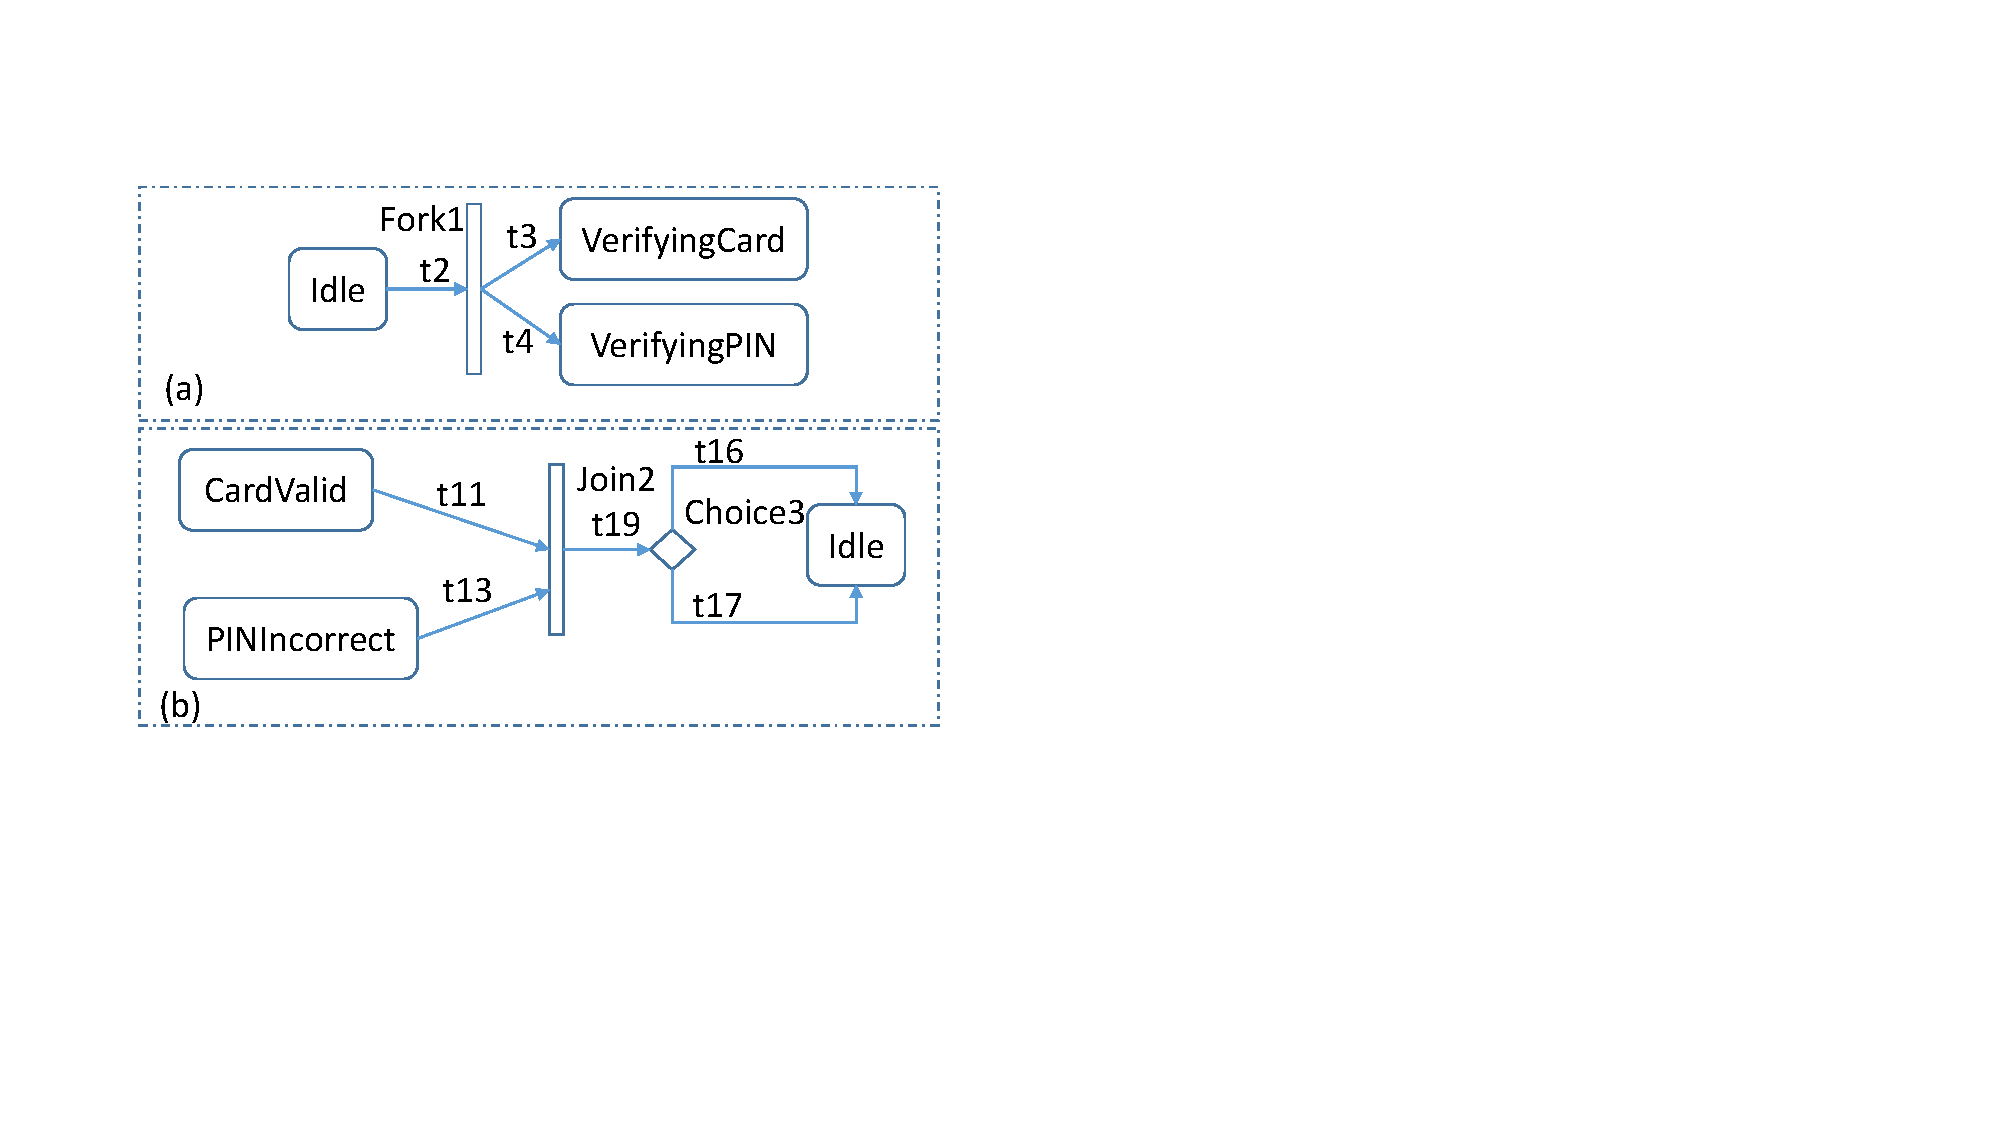
\includegraphics[clip, trim=2.0cm 6cm 17.5cm 3cm, width=\columnwidth]{figures/transitionGraph.pdf}
	\caption{Transition graphs} 
	\label{fig:transitionGraph}
\end{figure}


\begin{definition} A compound transition $t_{cp}$ is a virtual path which starts from one or multiple UML state and ends on one or multiple UML state. A compound transition is specified by a triple \{srcs($t_{cp}$), trc($t_{cp}$), tgts($t_{cp}$)\}, in which source part srcs($t_{cp}$) consists of one or multiple states, transition part trc($t_{cp}$) consists of multiple transitions, and target part tgts($t_{cp}$) consists of one or multiple states. 
\end{definition}


Given a state, Algorithm \ref{alg:cptransition} presents how to calculate transition graphs whose source $t_{cp}$ whose source part contains only a state $s$. 

\begin{algorithm}[]
	\caption{Transition graphs calculation
		\label{alg:cptransition}}
	\begin{algorithmic}[1]
		\Require{A state $s$ of a state machine}
		\Ensure{A set of transition graphs $\mathcal{GT}$}
		\Procedure{calculateTransGraphs}{$s$}
		\Let{$\mathcal{GT}$}{$\emptyset$} 
		\For {$out \in T_{outs}(s)$}
			\If {$tgt(out)$ is not a state}
				\Let{$\tau$}{($\mathcal{S}$, $\mathcal{L}$, $\mathcal{P}$, $\mathcal{T}$) $=\{\emptyset,\emptyset, \emptyset, \emptyset\}$}
				\Let{$\mathcal{P}$}{$\mathcal{P} \cup {tgt(out)}$}
				\Let{$\mathcal{S}$}{$\mathcal{S} \cup \{s\}$}
				\Let{$\mathcal{T}$}{$\mathcal{T} \cup {out}$}
				\If {$tgt(out).kind = join$}
					\Let{$ins$}{\\$\{i \in T_{ins}(tgt(out))| owner(src(i)) = owner(s)\}$}
					\Let{$\mathcal{S}$}{$\mathcal{S} \cup \{src(i)|i \in ins\}$}
					\Let{$\mathcal{T}$}{$\mathcal{T} \cup ins$}
				\EndIf
				\Let{$nexts$}{$FINDTRANS(tgt(out))$}
				\Let{$\mathcal{T}$}{$\mathcal{T} \cup nexts$}
				\Let{H}{\\$\{tgt(t)|t \in nexts \wedge tgt(t).kind = history\}$}
				\Let{$\mathcal{P}$}{$\mathcal{P} \cup \{src(t)|t \in nexts\} \cup H$}
				\Let{$\mathcal{L}$}{$\mathcal{L} \cup \{tgt(t)|t \in nexts \wedge tgt(t)$ is state $\}$}
								
				\Let{$\mathcal{GT}$}{$\mathcal{GT} \cup \{\tau\}$} 
			\EndIf
		\EndFor
		\EndProcedure
		
		\Require{A vertex $v$}
		\Ensure{Transition paths starting from $v$ and ending on a state}
		\Procedure{FindTrans}{$v$}
		\Let{$nextTrans$}{$T_{outs}(v)$}
		\For {$out \in T_{outs}(v)$}
			\If {$tgt(out)$ is not a state}
				\Let {$nextTrans$}{\\$nextTrans \cup FINDTRANS(tgt(out))$}
			\EndIf
		\EndFor	 			 	
		\Return {$nextTrans$} 
		\EndProcedure	
	\end{algorithmic}
\end{algorithm}

For example, applying this algorithm to all states of the state machine example in \ref{fig:example}, we can calculate other transition graphs which are:
\begin{IEEEeqnarray*}{lCr}
	\tau_{3} &=& (\mathcal{S}_3, \mathcal{L}_3, \mathcal{P}_3, \mathcal{T}_3) = (\{VerifyingCard\}, \{Idle, \\ 
	&& {} CardValid\}, \{Choice1\}, \{t5, t6, t7\}),
\end{IEEEeqnarray*}
\begin{IEEEeqnarray*}{lCr}	
	\tau_{4} &=& (\{VerifyingPIN\}, \{PINIncorrect, \\
	&& {} PINCorrect\}, \{Choice2\}, \{t8, t9, t10\}),
\end{IEEEeqnarray*} 
and
\begin{IEEEeqnarray*}{lCr}	
	\tau_{5} &=& (\{CardValid, PINCorrect\}, \{DispenseMoney\}, \\ 
	&& {} \{Join2\}, \{t12, t14, t15\}).
\end{IEEEeqnarray*} 

\end{comment}

\begin{comment}
\begin{definition} A transition graph $\tau$ is an acyclic directed graph ($\mathcal{T}_r$, $\mathcal{P}$, $\mathcal{T}$) where $\mathcal{P}$ is a set of vertexes, and $\mathcal{T}_{r}$ and $\mathcal{T}$ are sets of transitions. $\mathcal{T}_{r}$ is called the set of root transitions of the graph. Following conditions are satisfied:
	\begin{itemize}
		\item $\forall t \in \mathcal{T}_r, src(t)$ is a state.
		
		\item $\forall p \in \mathcal{P}, p.kind \notin \{state, comp, conc\}$.	
		
		\item $\forall t \in \mathcal{T}, src(t)$ is a pseudo state.
	\end{itemize}	
\end{definition}

A traversal from the root transitions of a transition graph to a stable state configuration is a compound transition. A state machine can contain multiple transition graphs. Fig. \ref{fig:transitionGraph} (a) and (b) show two transition graphs $\tau_{1}$ and $\tau_{2}$ of the ATM state machine, respectively, in which 
\begin{IEEEeqnarray*}{lCr}
	\tau_{1} &=& (\mathcal{T}_r, \mathcal{P}, \mathcal{T}) = (\{t2\}, \{Fork1\}, \{t3, t4\} )
\end{IEEEeqnarray*}
and
\begin{IEEEeqnarray*}{lCr}	
	\tau_{2} &=& (\{t11, t13\}, \{Join2, Choice3\}, \{t19, t16, t17\}).
\end{IEEEeqnarray*}



\begin{figure}
	\centering
	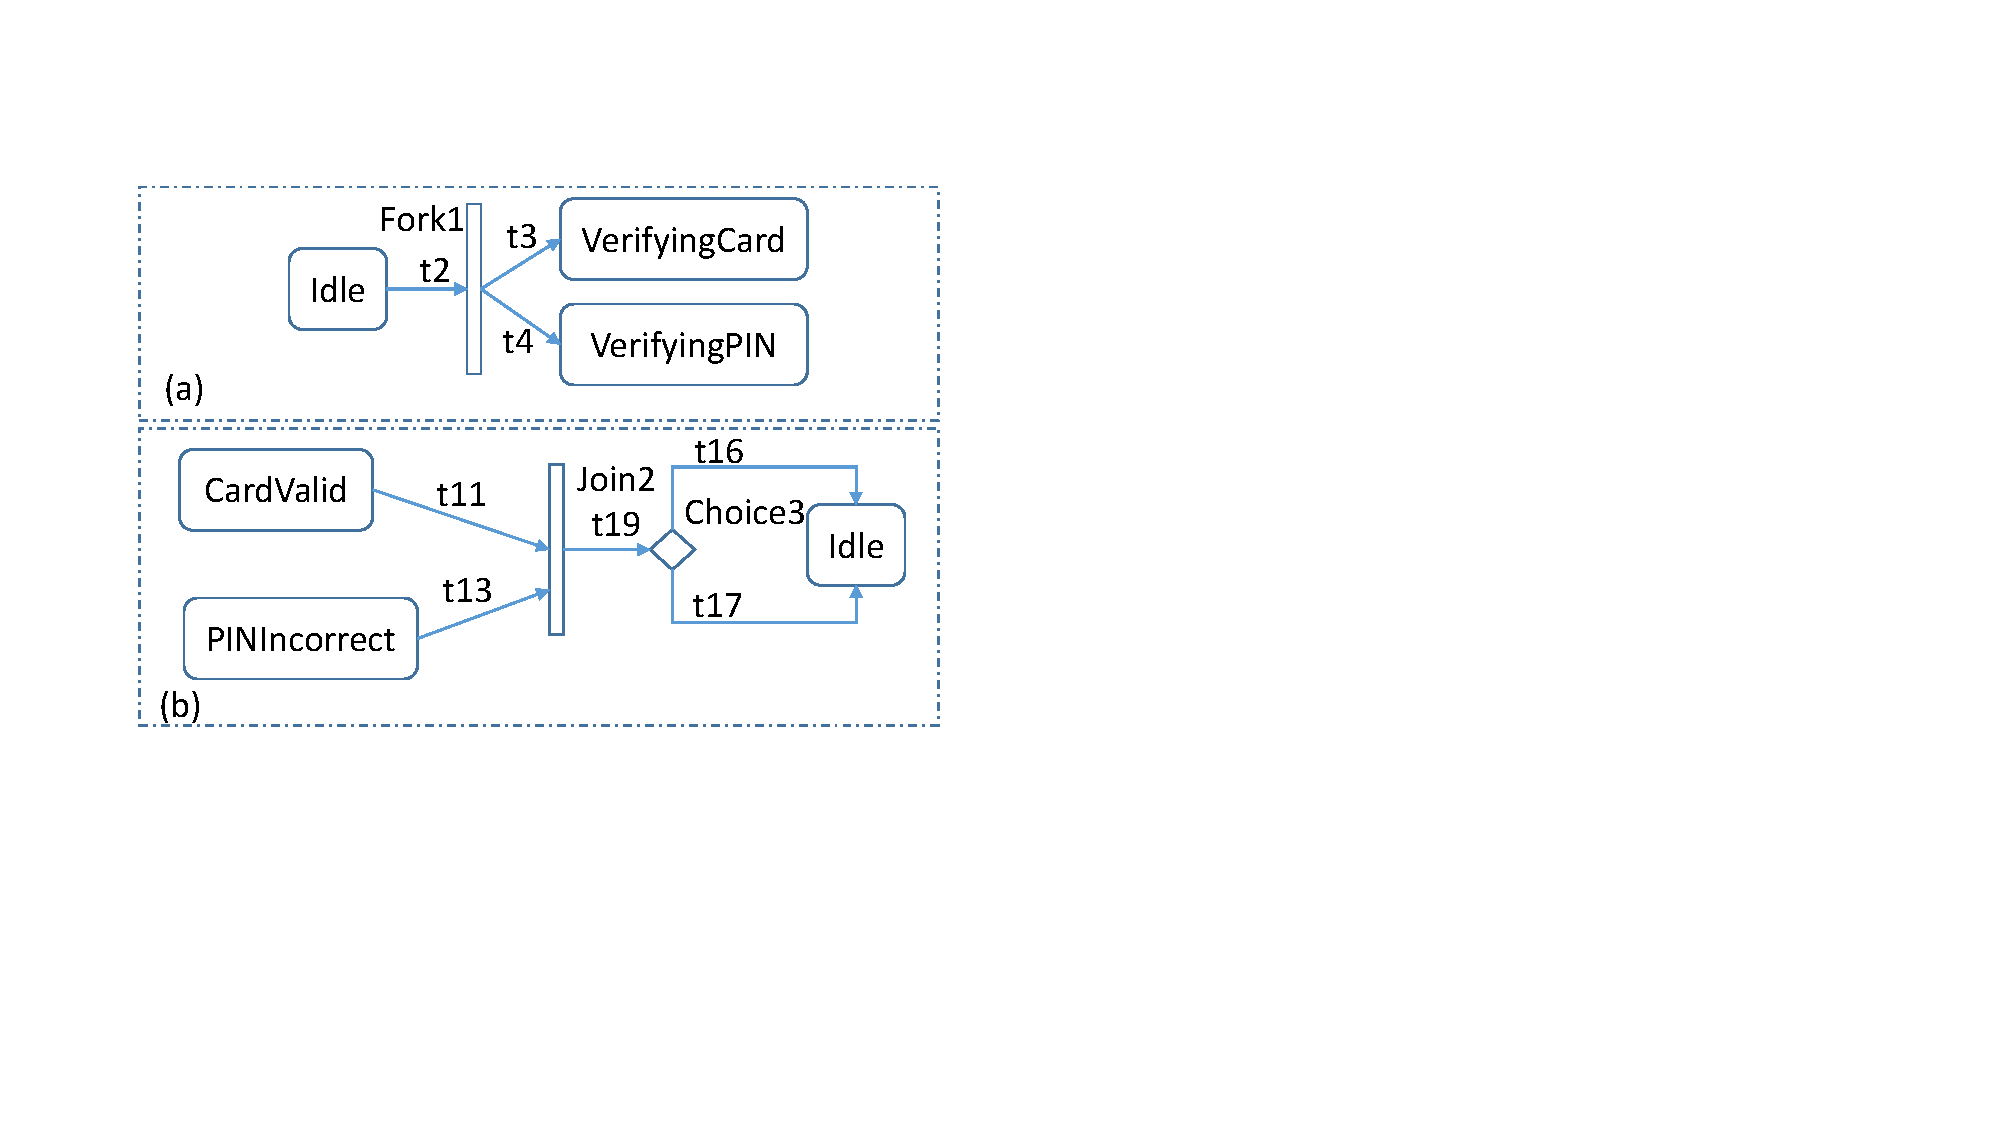
\includegraphics[clip, trim=2.0cm 6cm 17.5cm 3cm, width=\columnwidth]{figures/transitionGraph.pdf}
	\caption{Transition graphs} 
	\label{fig:transitionGraph}
\end{figure}



Given a state, Algorithm \ref{alg:cptransition} presents how to calculate transition graph set whose root transitions outgo from $s$. 

\begin{algorithm}[]
	\caption{Transition graphs calculation
		\label{alg:cptransition}}
	\begin{algorithmic}[1]
		\Require{A state $s$ of a state machine}
		\Ensure{A set of transition graphs $\mathcal{GT}$}
		\Procedure{calculateTransGraphs}{$s$}
		\Let{$\mathcal{GT}$}{$\emptyset$} 
		\For {$out \in T_{outs}(s)$}
			\If {$tgt(out)$ is not a state}
				\Let{$\tau$}{($\mathcal{T}_r$, $\mathcal{P}$, $\mathcal{T}$) $=\{\emptyset,\emptyset, \emptyset\}$}
				\Let{$\mathcal{P}$}{$\mathcal{P} \cup {tgt(out)}$}
				\Let{$\mathcal{T}_r$}{$\mathcal{T}_r \cup {out}$}
			\If {$tgt(out).kind = join$} 
				\Let{$\mathcal{T}_r$}{$\mathcal{T}_r \cup T_{ins}(tgt(out))$}
			\EndIf
				\Let{$nexts$}{$FINDTRS(tgt(out))$}
				\Let{$\mathcal{T}$}{$\mathcal{T} \cup nexts$}
			
				\Let{$\mathcal{GT}$}{$\mathcal{GT} \cup \{\tau\}$} 
			\EndIf
		\EndFor
		\EndProcedure
		
		\Require{A vertex $v$}
		\Ensure{Transition paths starting from $v$ to atomic  states}
		\Procedure{FINDTRS}{$v$}
		\Let{$outs$}{$T_{outs}(v)$}
		\For {$out \in T_{outs}(v)$}
			\If {$tgt(out)$ is not a state}
				\Let {$outs$}{\\$outs \cup FINDTRS(tgt(out))$}
			\ElsIf $tgt(out).kind \in {comp, conc}$
				\For {$sub \in subvertexes(tgt(out)), sub.kind=initial$}
					\Let {$outs$}{$outs \cup FINDTRS(sub)$}
				\EndFor
			\EndIf 
		\EndFor	 			 	
		\Return {$outs$} 
		\EndProcedure	
	\end{algorithmic}
\end{algorithm}

For example, applying this algorithm to all states of the state machine example in \ref{fig:example}, we can calculate other transition graphs which are:
\begin{IEEEeqnarray*}{lCr}
	\tau_{3} &=& (\mathcal{S}_3, \mathcal{L}_3, \mathcal{P}_3, \mathcal{T}_3) = (\{VerifyingCard\}, \{Idle, \\ 
	&& {} CardValid\}, \{Choice1\}, \{t5, t6, t7\}),
\end{IEEEeqnarray*}
\begin{IEEEeqnarray*}{lCr}	
	\tau_{4} &=& (\{VerifyingPIN\}, \{PINIncorrect, \\
	&& {} PINCorrect\}, \{Choice2\}, \{t8, t9, t10\}),
\end{IEEEeqnarray*} 
and
\begin{IEEEeqnarray*}{lCr}	
	\tau_{5} &=& (\{CardValid, PINCorrect\}, \{DispenseMoney\}, \\ 
	&& {} \{Join2\}, \{t12, t14, t15\}).
\end{IEEEeqnarray*} 


\begin{definition} Current active configuration $Cfg$ of a UML state machine sm is a set of candidate UML states which are able to process an incoming event. 
\end{definition}
\end{comment}

\subsection{Model-Driven Round-trip Engineering}
\label{subsec:mdrtebackground}

This section defines the actors in software development process who will use our model-code RTE technique to collaborate during development.
%Then we define the main capabilities, as use-cases, expected from a generic IDE used by these actors.
Some basic concepts related to the actors and use-cases, which will be offered by RAOES, are also defined in this section.


%\subsection{Collaborating actors and development artifacts}

%In this paper we propose a methodological model-code synchronization pattern for collaboration between software
%architects and programmers.

%First, we introduce the concepts of \textit{development artifact} and \textit{baseline artifact}.

%\begin{definition}[Development artifact]
%	A development artifact is an artifact, as defined in \cite{omg_software_2008},
%	that can be used for the full implementation of the system.
%\end{definition}

%For example a system can be entirely implemented as code.
%Implementation code is a development artifact, so may model.
%It is then not only documentation of specification
%but part of the implementation.
%For example a model can be used for implementation by generating code from the model, and compiling the code without the need to edit or complete the code.
%In our work, we assume that model and code are both development artifacts.
%A development artifact may be the baseline artifact, defined in this paper as follows:

\begin{comment}

\begin{definition}[Baseline artifact]
	A baseline artifact is one which may be edited manually.
	All other artifacts are produced from the baseline artifact
	through some process, and only through a process. Manual edition
	of artifacts other than the baseline artifact is forbidden.
\end{definition}
\end{comment}

Two primary actors, called \ttt{model-driven developer}
and \ttt{code-driven developer}, are introduced.
%The main difference between them
%is what they consider as the baseline artifact.

\begin{definition}
	A model-driven developer (MDD) is an actor who uses the model as the main working artifact. Code-driven developer (CDD) is an actor who uses the code as the main working artifact.
\end{definition}

%In other words, for the model-driven developer only the model should be edited manually. 
The code, produced from the model automatically, is consistent with the model.
A software architect is a kind of the model-driven developer
who edits the model to specify the system architecture.
%An architect presumes that the reference for the architecture
%of the system should be specified as a model.



A programmer is a specialization of the code-driven developer.
Indeed, programmers may modify our C++ front-end code, such as editing methods, attributes or state machines textually.
%The code is then the main reference for the implementation of methods.

%There are some use-cases for manual edition of artifacts. The \texttt{Edit Artifact} use-case
%implies that the IDE must have some tool to let the developer manually edit an artifact.
%The \texttt{Edit Model} and \texttt{Edit Code} use-cases are specializations of the \texttt{Edit Artifact}
%use-case where the artifact is the model or code.

%There are also some use-cases related to the synchronization of artifacts. The \texttt{Synchronize Artifact} use-case (1) compares two artifacts, (2) updates each with editions made
%in the related artifact, and (3) reconciles conflicts when appropriate. The \texttt{Synchronize Model} and \texttt{Synchronize Code}
%use-cases are specializations where, respectively, the model or the code are the artifacts being synchronized.

\texttt{Generate Code} is a use-case related to forward engineering.
It is the production of C++ code from a model.
The developer can either use \texttt{Generate Code (Batch)} or \texttt{Generate Code (Incremental)}.
%\end{comment}

\begin{definition}[Batch code generation] \ttt{Batch code generation} \cite{Giese2006} is a process of generating code
	from a model, from scratch.
	Any existing code is overwritten by the newly generated code.
\end{definition}

%\ttt{Incremental code generation} is a specialization of \ttt{incremental model transformation}, which
%does not generate the whole target model from scratch but only updates the target model by
%propagating editions made to the source model.

%\texttt{Incremental code generation (ICG)} \ti{$gen_{inc}$ is a process of taking as input a changed model m and an existing executable code to make the code synchronized with the changed model: $gen_{inc}(m, c) = c'$. Non-conflicted changes at the code side are kept intact the synchronization. ICG is also defined as a process of taking model changes ch and an existing code c: $gen_{inc}(ch, c) = c'$}.

%Derived from the definition of incremental model transformation, 
%Incremental code generation
%is defined in this paper as follows:

\begin{definition}[Incremental code generation]
	\ttt{Incremental code generation} is the process
	of taking as input an edited model and existing code to update the code by propagating
	editions in the model to the code.
\end{definition}

%\begin{comment}
\texttt{Reverse Code} is related to reverse engineering.
\texttt{Reverse Code} is the production of a model, in a modeling language such as UML, from code, written in a programming language.
The developer can either use \texttt{Reverse Code (Batch)} or \texttt{Reverse Code (Incremental)}, which are defined in this paper as follows:
%\end{comment}

\begin{definition}[Batch reverse engineering]
	\ttt{Batch reverse engineering} is a process of producing a model from code, from scratch.
	The existing model is overwritten by the newly produced model.
\end{definition}

\begin{definition}[Incremental reverse engineering]
	\ttt{Incremental reverse engineering} is the process of taking as
	input a edited code, and an existing model, and then updating the model by propagating
	editions in the code to the model.
\end{definition}

%For readability, in this paper we will sometimes designate batch and incremental as modes
%of code generation/reverse; e.g. we say that we generate code in batch mode from a model.

%The use-cases are generic. They do not depend
%on any particular approach or tool. Therefore the software developers
%can choose the approach or tool that suits better his/her
%development preferences best.

In Section \ref{sec:collaboration}, the use-cases are integrated into
our process, which covers model-code synchronization and is detailed in Section \ref{sec:collaboration}.
%The scenarios correspond to behaviors performed by both kinds of actors,
%i.e. model-driven developers and code-driven developers.

%Model-driven engineering has been established as a potential approach to gain software quality and productivity \cite{Mussbacher2014}. 




